\documentclass[noheader]{coursclass}


\begin{document}

\begin{center}
	\begin{tikzpicture}[scale=0.95,every node/.style={scale=0.85}]
		\draw (0,0) ellipse (2 and 1);
		\draw (0,0.5) ellipse (3.7 and 2);
		\draw (0,1) ellipse (5.4 and 3);
		\draw (0,1.5) ellipse (7.1 and 4);
		\draw (0,2) ellipse (8.8 and 5);

		\node at (0,0.7) {$ℕ$};
		\node at (-0.9,0.1) {$0$};
		\node at (0,0.1) {$1$};
		\node at (0.9,0.1) {$2$};
		\node at (-0.6,-0.5) {$50$};
		\node at (0.6,-0.5) {$357$ $892$};

		\node at (0,2.2) {$ℤ$};
		\node at (-1,1.7) {$-1$};
		\node at (1.2,1.7) {$-76$};
		\node at (-2.5,0.5) {$-2689$};

		\node at (0,3.7) {$𝔻$};
		\node at (-3,2.7) {$0{,}8$};
		\node at (2,2.8) {$-89{,}127$};

		\node at (0,5.2) {$ℚ$};
		\node at (-6,2) {$-\frac{6}{11}$};
		\node at (-3,4) {$\frac{1}{3}$};
		\node at (5,3.5) {$\frac{60}{859}$};

		\node at (0,6.7) {$ℝ$};
		\node at (-5,5) {$\sqrt{3}$};
		\node at (-2,6) {$\sqrt{2}$};
		\node at (3,6) {$π$};
		\node at (8,3) {$e$};
	\end{tikzpicture}
\end{center}

\begin{exemple}
	\begin{itemize}
		\item Exemple d'entiers naturels : $0$ ; $1$ ; $2$ ; $50$ ; $357$ ; $892$ ...
		\item Exemple d'entiers relatifs mais pas naturels : $-1$ ; $-76$ ; $-2689$ ...
		\item Exemple de nombres décimaux mais pas d'entiers relatifs : $0,8$ ; $-89,127$ ...
		\item Exemple de nombres rationnels mais pas décimaux : $\dfrac{6}{11}$ ; $\dfrac{1}{3}$ ; $\dfrac{60}{859}$ ...
		\item Exemple de nombres réels mais pas rationnels : $\sqrt{2}$ ; $\sqrt{3}$ ; $π$ ; $e$ ...
	\end{itemize}
\end{exemple}

\vspace{2em}

\begin{definition}[Intervalle de $ℝ$]
	Soient $a$ et $b$ deux nombres réels tels que $a ≤ b$.
	\begin{itemize}
		\item L'\textbf{intervalle} $[a ; b]$ est l'ensemble des nombres réels $x$ tels que $x ≥ a$ et $x ≤ b$.

		      On dit que $a$ et $b$ sont les \textbf{bornes} de cet intervalle.

		      L'\textbf{amplitude} de cet intervalle est $b - a$.
		\item L'\textbf{intervalle} $]-∞ ; b]$ est l'ensemble des nombres réels $x$ tels que $x ≤ b$.
		\item L'\textbf{intervalle} $[a ; +∞[$ est l'ensemble des nombres réels $x$ tels que $x ≥ a$.
	\end{itemize}

	Pour exclure une des bornes d'un intervalle, il faut utiliser un crochet tourné vers l'extérieur.

	Ainsi $[a ; b[$ est l'ensemble des nombres réels $x$ tels que $x ≥ a$ et $x < b$.
\end{definition}

\begin{exemple}
	\begin{center}
		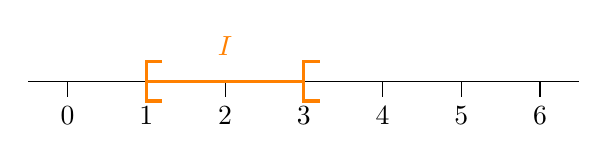
\begin{tikzpicture}
			\draw[\myArrow] (-0.5,0) -- (6.5,0);
			\foreach \x in {0,...,6} {
					\draw (\x,0) -- ++(0,-0.2) node[below] {$\x$};
				}
			\draw[very thick,orange]
			(1,0) -- (3,0)
			(1.2,0.25) -- ++(-0.2,0) -- ++(0,-0.5) -- ++(0.2,0)
			(3.2,0.25) -- ++(-0.2,0) -- ++(0,-0.5) -- ++(0.2,0);
			\node[orange,above] at (2,0.2) {$I$};
		\end{tikzpicture}
	\end{center}

	Sur la droite ci-dessus, $I$ est l'intervalle \correctionDots{$[1, 3[$}.

	Ainsi :
	\begin{itemize}
		\item $I$ contient par exemple \correctionDots{$1$, $2$ ou encore $1,5$.}
		\item $I$ ne contient pas par exemple \correctionDots{$3$, $0$ ou encore $5,6$.}
	\end{itemize}
\end{exemple}

\end{document}